% Standalone pgfplots figure -- compile with pdflatex/lualatex,
% or \input{} into a doc that loads \usepackage{pgfplots}.
% Bivariate-bicycle FILTERED memory_Z (basis Z), p-bit decoder, t_v=5.
\documentclass[tikz,border=3mm]{standalone}
\usepackage{pgfplots}
\pgfplotsset{compat=1.17}
\begin{document}
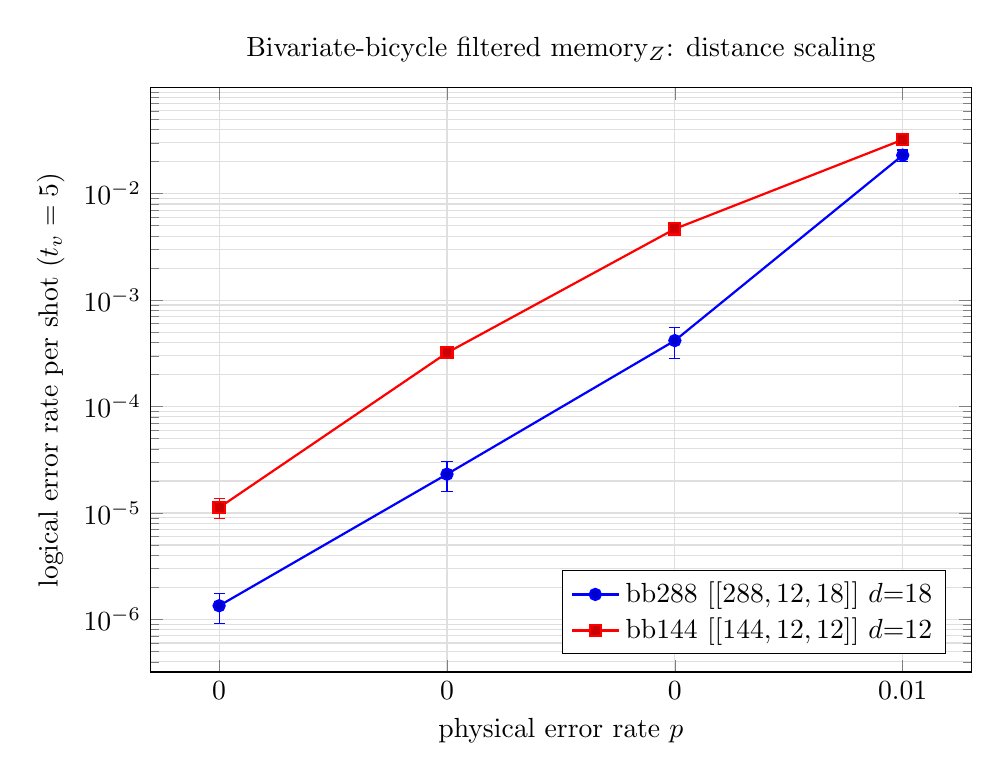
\begin{tikzpicture}
\begin{semilogyaxis}[
    width=12cm, height=9cm,
    xlabel={physical error rate $p$},
    ylabel={logical error rate per shot ($t_v=5$)},
    title={Bivariate-bicycle filtered memory$_Z$: distance scaling},
    xtick={0.002,0.003,0.004,0.005},
    scaled x ticks=false, x tick label style={/pgf/number format/fixed},
    grid=both, grid style={gray!25},
    legend pos=south east, legend cell align=left,
    mark options={solid}, every axis plot/.append style={thick},
]
\addplot+[color=blue, mark=*, error bars/.cd, y dir=both, y explicit]
    coordinates {(0.002, 1.3441e-06) +- (0, 4.2504e-07) (0.003, 2.3148e-05) +- (0, 7.3201e-06) (0.004, 4.1667e-04) +- (0, 1.3176e-04) (0.005, 2.3000e-02) +- (0, 2.7689e-03)};
\addlegendentry{bb288 $[[288,12,18]]$ $d{=}18$}
\addplot+[color=red, mark=square*, error bars/.cd, y dir=both, y explicit]
    coordinates {(0.002, 1.1230e-05) +- (0, 2.3417e-06) (0.003, 3.2031e-04) +- (0, 2.8882e-05) (0.004, 4.6719e-03) +- (0, 2.7018e-04) (0.005, 3.2188e-02) +- (0, 2.2426e-03)};
\addlegendentry{bb144 $[[144,12,12]]$ $d{=}12$}
\end{semilogyaxis}
\end{tikzpicture}
\end{document}
